\chapter{Augmentation der generierten Bilder}

\label{chap:5}

Wie bereits erwähnt ist das Ziel dieser Studienarbeit nicht alleine die Generierung von Bildern, die Straßenschilder zeigen. Zusätzlich soll die Arbeit einige der in Kapitel \ref{chap:stand-der-technik-strassenschilderkennung} genannten Probleme für die Straßenschilderkennung simulieren. Das Skript \mintinline{python}{generate.py} erlaubt deshalb die Methoden der Augmentierung, die bereits in Tabelle \ref{tab:generate-cli} aufgeführt sind. Diese sind eine \textbf{Bewegungsunschärfe}, das Hinzufügen von \textbf{Schnee} und das \textbf{markieren von Schildern als ungültig}. Dafür dient ein Modul \mintinline{python}{utils.image_augmentation}. Für jede der Augmentierungen befinden sich Beispiel-Abbildungen im Anhang.

Die Augmentierung ist weitgehend prozedural implementiert, da keine ausreichend großen Datensätze bekannt sind, die solche Grenzfälle der Straßenschilderkennung zeigen. Diese wären als Trainingsgrundlage für das \ac{CycleGAN} notwendig.

\section{Bewegungsunschärfe}
\label{sec:motion-blur}
Verwackelte Bilder können insbesondere dann entstehen, wenn sich das Fahrzeug mit einer hohen Geschwindigkeit bewegt. Hierbei entsteht eine Bewegungsunschärfe. Dies tritt bei einer Kamera auf, wenn sich das Bild während der Belichtungszeit deutlich verändert. Wenn also die Geschwindigkeit des Fahrzeugs groß ist im Vergleich zur Belichtungszeit. Da sich das fotografierte Objekt zu unterschiedlichen Zeitpunkten an verschiedenen Positionen im Bild befindet, erscheint es als verschwommen. Während bei der Straßenschilderkennung eine Bewegungsunschärfe die Erkennung erschwert, existieren Bereiche, in denen Fotografen absichtlich versuchen sie zu erzeugen. Dazu zählt beispielsweise die Sportfotografie, in der Objekte schneller erscheinen, wenn sie verschwommen zu sehen sind. Die Literatur gibt jedoch Hinweise darauf, dass es nicht trivial sei, die Bewegungsunschärfe mit einer Kamera exakt zu steuern. Beispielsweise wenn die Unschärfe eine bestimmte Intensität haben soll. Aus diesem Grund besteht Interesse daran, Bewegungsunschärfe computergestützt zu erzeugen. \cite{motion-blur}

Ähnlich zu der Funktionsweise von \acp{CNN} basiert die küstliche Erzeugung von Bewegungsunschärfe auf einer Faltung des Bilds mit einer Faltmatrix. Die Idee ist, jeden Pixelwert durch einen Durchschnitt der umliegenden Pixelwerte zu ersetzen. Dabei jedoch linear entlang einer bestimmten Richtung, um eine lineare Bewegung zu simulieren. Je mehr Pixel in die Berechnung des Durchschnitts einbezogen werden, desto stärker erscheint die Bewegungsunschärfe. Die Bewegungsunschärfe in dieser Studienarbeit ist entweder horizontal, vertikal oder diagonal. Es ergeben sich dadurch drei Arten von Faltmatrizen, die in Abbildung \ref{fig:faltmatrizen} gezeigt sind. \cite{motion-blur}

\begin{figure}[h]
	\centering
	\begin{tikzpicture}[baseline=(current bounding box.center)]
		\matrix (A) [nodes={draw, minimum size=9mm}, column sep=-0.2mm] {
			\node{0}; & \node{0}; & \node{0}; \\
			\node{$0.\bar{3}$}; & \node{$0.\bar{3}$}; & \node{$0.\bar{3}$}; \\
			\node{0}; & \node{0}; & \node{0}; \\
		};
		\matrix (B) [nodes={draw, minimum size=9mm}, column sep=-0.2mm, right= of A] {
			\node{0}; & \node{$0.\bar{3}$}; & \node{0}; \\
			\node{0}; & \node{$0.\bar{3}$}; & \node{0}; \\
			\node{0}; & \node{$0.\bar{3}$}; & \node{0}; \\
		};
		\matrix (C) [nodes={draw, minimum size=9mm}, column sep=-0.2mm, right= of B] {
			\node{$0.\bar{3}$}; & \node{0}; & \node{0}; \\
			\node{0}; & \node{$0.\bar{3}$}; & \node{0}; \\
			\node{0}; & \node{0}; & \node{$0.\bar{3}$}; \\
		};
	\end{tikzpicture}
	\caption{Horizontale, vertikale und diagonale Faltmatrix}
	\label{fig:faltmatrizen}
\end{figure}

Die Größe der Faltmatrix gibt die Stärke der Unschärfe an. Bei einer größeren Faltmatrix fließen nämlich mehr Pixel in die Berechnung des Durchschnitts ein. Da die Faltung hier jeden Pixel gleich stark gewichtet, sind alle Parameter der Faltmatrix entlang der simulierten Bewegungsrichtung identisch. Damit jeder Pixel dieselbe Helligkeit besitzt, müssen die Parameter zudem zusammen den Wert \emph{eins} ergeben \cite{motion-blur}. Das ist der Grund, wieso die 3x3-Matrizen in Abbildung \ref{fig:faltmatrizen} die Werte $0.\bar{3}$ haben. Eine 4x4-Matrix hingegen hätte die Werte $0.25$. In dem Modul \mintinline{python}{utils.image_augmentation} existiert die Funktion \mintinline{python}{apply_motion_blur} um auf einen einzelnen Bild-Tensor der Stufe drei eine Bewegungsunschärfe auszuführen. Zusätzlich besitzt die Funktion verschiedene Parameter zur Steuerung der Intensität und der Richtung des Effekts. Listing \ref{code:motion-blur} zeigt, wie die Funktion die Bewegungsunschärfe in diagonaler Richtung durchführt.

\begin{code}
  \begin{minted}{python}
  kernel = np.identity(kernel_size)
  kernel = kernel / kernel_size
  transformed_img = cv2.filter2D(img_tensor.numpy(), -1, kernel)
  \end{minted}
  \caption{\lstinline[language=python]{utils.image_augmentation.py} - Hinzufügen einer diagonalen Bewegungsunschärfe}
  \label{code:motion-blur}
\end{code}

Die Variable \mintinline{python}{kernel} steht für die Faltmatrix. Numpy besitzt eine Funktion \mintinline{python}{identity}, die eine Einheitsmatrix erzeugt. Diese Matrix besitzt auf der Hauptdiagolen Einsen und sonst Nullen. Die \mintinline{python}{kernel_size} gibt die Größe der Matrix an. Damit alle Werte der Matrix summiert den Wert \emph{eins} ergeben, teilt die Funktion die Matrix durch die \mintinline{python}{kernel_size}. In der letzten Codezeile in Listing \ref{code:motion-blur} faltet die Funktion \mintinline{python}{apply_motion_blur} das Eingangsbild mit der Faltmatrix. Dazu nutzt sie die Funktion \mintinline{python}{filter2D} aus der OpenCV Bibliothek. Die Funktion wird genutzt, da sich keine TensorFlow Funktion hat finden lassen, mit der eine derart definierte Faltmatrix auf einem Bild angewendet werden kann, ohne Convolutional Layer zu verwenden. Die Funktion erhält drei Parameter: Den Bild-Tensor, jedoch konvertiert in ein Numpy Array, den Wert $-1$ und die Faltmatrix. Der Wert $-1$ gibt an, dass die Funktion die Anzahl an Farbkanälen des Bilds beibehalten soll.

\section{Ungültige Straßenschilder}
In Kapitel \ref{chap:stand-der-technik-strassenschilderkennung} ist bereits beschrieben, dass als ungültig markierte Schilder eine Herausforderung für heutige Straßenschilderkennungen darstellen können. Aus diesem Grund implementiert diese Studienarbeit den Anwendungsfall. Ungültige Schilder sind im Straßenverkehr meist durch ein orangefarbenes Kreuz gekennzeichnet.

Bei der Umsetzung bieten sich verschiedene Möglichkeiten. Zum einen kann das \ac{CycleGAN} darauf trainiert werden, solche Bilder eigenständig zu generieren. Dafür benötigt das Modell Trainingsdaten mit ungültigen Schildern. Der Datensatz müsste somit um reale Bilder ergänzt werden, was nicht ohne weiteres möglich ist. Es wäre jedoch auch denkbar, bereits vorhandene Trainingsbilder mit einer Bildbearbeitungssoftware so anzupassen, dass sie ungültige Schilder zeigen.

Eine weitere Möglichkeit ist, das Kreuz, das die Ungültigkeit eines Schilds markiert, nachträglich in die generierten Bilder des \ac{CycleGAN} einzufügen. Die Besonderheit ist hierbei, dass die Straßenschilder zufällig rotiert und skaliert sind. Die Augmentierungsfunktion muss das Kreuz vorher so transformieren, dass es sich stets zentral und mit einer angepassten Rotation auf dem Schild befindet. Da hierfür keine zusätzlichen Trainingsdaten nötig sind, implementiert das Modul  \mintinline{python}{utils.image_augmentation} dieses Vorgehen. Die Funktion dafür heißt \mintinline{python}{make_street_sign_invalid}. 

Für zukünftige Arbeiten ist ein weiterer Ansatz, die Kreuze vor der Bild-zu-Bild Generierung auf die Piktogramme einzufügen. Dafür können Entwickelnde die Funktion \mintinline{python}{make_street_sign_invalid} verwenden. Sie müssen das entstehende Bild anschließend skalieren und rotieren und an das \ac{CycleGAN} als Eingangsdomäne $X$ übergeben. Auch hierfür benötigt das Modell zusätzliche Trainingsdaten. Es muss jedoch nicht von alleine lernen, das Kreuz zu erzeugen, da dies bereits im Eingangsbild enhalten ist. Außerdem kann der Quellcode genutzt werden, um andere Objekte auf die Schilder einzufügen. Beispielsweise wenn Entwickelnde das \ac{CycleGAN} erweitern wollen, um Vandalismus auf Straßenschildern zu simulieren.

In dem Ordner \mintinline{python}{Augmentation} unter \href{https://drive.google.com/drive/folders/11gaUErheUYb0WlBPtWhxgCK7mE0URHYI?usp=sharing}{\textbf{dem Link des Datensatzes}} (Stand: 09.06.2023) befindet sich das rohe Bild eines orangefarbenen Kreuzes auf einem transparenten Hintergrund. Abbildung \ref{fig:cross} zeigt dieses Bild.
\begin{figure}[h]
	\centering
	\includegraphics[width=0.15\textwidth]{images/augmented images/cross.png}
	\caption{Kreuz auf transparentem Hintergrund, das Schilder als ungültig kennzeichnet}
	\label{fig:cross}
\end{figure} 
Prinzipiell implementiert die Funktion \mintinline{python}{make_street_sign_invalid} folgendes: Sie augmentiert das Bild genau wie das übergebene Straßenschild und fügt es dann auf das Schild ein. Aufrufende Funktionen müssen deshalb nicht nur ein generiertes Schild übergeben, sondern auch den Wert für die Skalierung sowie die Transformationsmatrix, die zu diesem generierten Bild geführt hat. Die Funktion \mintinline{python}{make_street_sign_invalid} kann das Kreuz dann mit den gleichen Parametern skalieren und rotieren wie das Straßenschild. Dadurch fügt die Funktion das Kreuz zentriert auf das Straßenschild ein. Die Funktion \mintinline{python}{make_street_sign_invalid} besteht in verkürzter Form aus dem Code in Listing \ref{code:invalid-sign}.

\begin{code}
	\begin{minted}{python}
cross = preprocess_image.transform_image(cross, content_size, 
		transformation_matrix, bg_is_white=False)
img_tensor = tf.concat([img_tensor, 
		tf.ones_like(img_tensor[:, :, 0:1])], axis=-1)
# img_tensor and cross are numpy arrays here
img_tensor.paste(cross, (0, 0), cross)
	\end{minted}
	\caption{\lstinline[language=python]{utils.image_augmentation.py} - Schilder als ungültig markieren}
	\label{code:invalid-sign}
\end{code}

Die Variable \mintinline{python}{cross} ist ein Bild-Tensor der Stufe drei, der das Kreuz enthält. Dabei hat der Tensor jedoch nicht wie in dieser Studienarbeit üblich die Form \emph{(256, 256, 3)} sondern \emph{(256, 256, 4)}. Das liegt daran, dass jeder der $256\cdot 256$ Pixel zusätzlich zu den Werten für rot, grün und blau auch einen \emph{Alphakanal} besitzt. Dieser gibt an, wie transparent der Pixel ist. Der Wert $0$ bedeutet, dass der Pixel vollständig transparent ist, während der Wert $1$ bedeutet, dass der Pixel vollständig deckend ist. Der transparente Hintergrund um das Kreuz besitzt damit überall einen Alpha-Wert von $0$. In der ersten Codezeile in Listing \ref{code:invalid-sign} wird das Bild des Kreuzes augmentiert. Dazu wird die gleiche Funktion genutzt wie für die Datenaugmentierung des \ac{CycleGAN}: \mintinline{python}{transform_image} aus \mintinline{python}{utils.preprocess_image}. Neben dem Tensor \mintinline{python}{cross} übergibt die Funktion hier die beiden Transformationsgrößen sowie den Parameter \mintinline{python}{bg_is_white=False}. Damit füllt die Funktion \mintinline{python}{tranform_image} den Hintergrund des Bilds mit vollständig transparenten statt mit weißen Pixeln auf.

In einem nächsten Schritt fügt die Funktion dem generierten Eingangsbild \mintinline{python}{img_tensor} einen Alphakanal mit den Werten $1$ hinzu. Dafür existiert die Funktion \mintinline{python}{tf.concat}, die mehrere Tensoren zusammenfügen kann. Einer ihrer Parameter ist eine Liste von Tensoren, die miteinander konkateniert werden sollen. Der erste Tensor ist der Eingangstensor der Form \emph{(256, 256, 3)}. Der zweite Tensor hat die Form \emph{(256, 256, 1)} und enthält nur Einsen als Werte. Der Code \mintinline{python}{img_tensor[:, :, 0:1]} entnimmt aus dem Eingangsbild einen einzelnen Farbkanal, während die Funktion \mintinline{python}{tf.ones_like} diesen Farbkanal komplett mit Einsen auffüllt. Der Parameter \mintinline{python}{axis=-1} legt fest, dass der neu erzeugte Alphakanal an die letzte Achse des Tensors angefügt wird, an der sich die Farbkanäle befinden. Der so erzeugte Tensor hat die Form \emph{(256, 256, 4)} und enthält neben den Farbwerten auch einen Alphakanal.

Das Bild wird dadurch nicht verändert, da beide Bilder nun die gleiche Anzahl an Farbkanälen haben, kann die Funtkion \mintinline{python}{make_street_sign_invalid} das Kreuz jedoch nun auf das Eingangsbild einfügen. Dazu dient die Funktion \mintinline{python}{paste} aus der Bibliothek Pillow. Sie fügt das Kreuz an die Koordinaten $(0,0)$ ein. Der dritte Parameter mit dem Wert \mintinline{python}{cross} sorgt dafür, dass die transparenten Pixel des Kreuzes erhalten bleiben und damit das Eingangsbild nicht überdecken. Vor der Anwendung der Pillow-Funktion werden die Bilder in Numpy Arrays konvertiert. \cite{pillow}

\section{Schnee}

Schnee ist eine Wetterbedingung, die, ausgehend von Kapitel \ref{chap:stand-der-technik-strassenschilderkennung}, eine Auswirkung auf die Straßenschilderkennung haben kann. Es ließen sich keine Veröffentlichungen finden, die das künstliche Einfügen von Schnee auf Bilder in eine in diesem Rahmen umsetzbare Art und Weise aufzeigen. Aus diesem Grund basiert die Implementierung auf folgendem Vorgehen: Ein Bildbearbeitungsprogramm wurde genutzt, um ein Bild aus künstlichem Schnee zu erstellen. Anschließend daran wurde das Vorgehen in dem Bildbearbeitungsprogramm als ein Algorithmus formuliert, der das Vorgehen in Python automatisieren kann.

Der Algorithmus besteht aus folgenden Schritten:
\begin{enumerate}
  \item Erstelle ein Bild, das aus zufälligen schwarzen und weißen Pixeln besteht. Die Anzahl an weißen Pixel soll kleiner sein als die der schwarzen Pixel.
  \item Führe auf dem Bild ein gaußsches Weichzeichen aus. Hierdurch verschmieren die einzelnen weißen Pixel zu größeren Punkten.
  \item Führe auf dem Bild eine Bewegungsunschärfe aus. Dadurch wird die Bewegung der Schneeflocken entlang einer Windrichtung simuliert.
  \item Mache den schwarzen Hintergrund transparent und füge das erstellte Bild auf ein generiertes Straßenschild-Bild ein.
\end{enumerate}

Die Funktion \mintinline{python}{add_snow} implementiert diesen Algorithmus. Sie erzeugt die zufälligen schwarzen und weißen Pixel mittels einer Binomialverteilung. Für jeden Pixel existieren zwei Mögliche \emph{Ziehungen} aus der Verteilung: Schwarz (0) oder weiß (1). Ein $p$ gibt an, wie hoch die Wahrscheinlichkeit dafür ist, dass ein weißer Pixel gezogen wird. Die Problemstellung lässt sich für jeden Pixel als ein Zufallsexperiment mit zwei möglichen Ausgängen beschreiben. Das ist der Grund, wieso die Funktion hier eine Binomialverteilung implementiert. Dafür bietet TensorFlow die Funktion \mintinline{python}{tf.random.stateless_binomial}. Das auf dem Bild ausgeführte gaußsche Weichzeichen sorgt dafür, dass jeder Pixel \emph{verschwommen} wird. Das kann mit dem vorgehen für die Bewegungsunschärfe verglichen werden. Mit dem Unterschied, dass die Unschärfe hier nicht linear in eine Richtung zeigt, sondern kreisförmig um jeden Pixel ist. Damit wird aus jedem weißen Pixel ein kreisförmiger Punkt, der eine Schneeflocke darstellen soll. Für das gaußsche Weichzeichen bietet die Bilbiothek TensorFlow Addons die Funktion \mintinline{python}{tfa.image.gaussian_filter2d}. Für die anschließende Bewegungsunschärfe ruft die Funktion \mintinline{python}{add_snow} die in Abschnitt \ref{sec:motion-blur} beschriebene Funktion \mintinline{python}{add_motion_blur} auf. \cite{geometric-ops}

Diese Augmentierung der Bilder ist zusätzlich für eine weitere Fragestellung genutzt: \textbf{\emph{Kann das \ac{CycleGAN} lernen, verschneite Bilder eigenständig zu generieren?}}. Dazu existiert eine \emph{Checkpoint}-Datei, die Parameter des U-Net-Modells enthält, wenn es auf verschneiten Bildern trainiert ist. In dem \href{https://drive.google.com/drive/folders/11gaUErheUYb0WlBPtWhxgCK7mE0URHYI?usp=sharing}{\textbf{Link des Datensatzes}} befinden sich die Trainingsbilder unter dem Pfad \mintinline{python}{'Train with Snow'}.

Die Basis für das Training stellt das für 200 Epochen trainierte U-Net-basierte \ac{CycleGAN} dar. Auf den verschneiten Bildern ist das Modell zusätzliche 20 Epochen trainiert. Abbildung \ref{fig:snow-imgs-training} zeigt den Verlauf des Trainings. Die Bilder stammen aus verschiedenen Trainingsepochen, wobei das erste Bild zu der ersten Epoche korrespondiert und das letzte Bild zu der zwangigsten Epoche.

\begin{figure}[H]
	\centering
  \captionsetup[subfigure]{labelformat=empty}
	\begin{subfigure}[b]{0.125\textwidth}
		 \centering
		 \includegraphics[height=\textwidth]{../images/snow generation/training/1.png}
	\end{subfigure}
	\hspace{0.5em}%
	\begin{subfigure}[b]{0.125\textwidth}
		 \centering
		 \includegraphics[height=\textwidth]{../images/snow generation/training/2.png}
	\end{subfigure}
	\hspace{0.5em}%
	\begin{subfigure}[b]{0.125\textwidth}
		 \centering
		 \includegraphics[height=\textwidth]{../images/snow generation/training/6.png}
	\end{subfigure}
	\hspace{0.5em}%
	\begin{subfigure}[b]{0.125\textwidth}
	 \centering
	 \includegraphics[height=\textwidth]{../images/snow generation/training/8.png}
  \end{subfigure}
  \hspace{0.5em}%
  \begin{subfigure}[b]{0.125\textwidth}
	\centering
	\includegraphics[height=\textwidth]{../images/snow generation/training/11.png}
	\end{subfigure}
	\hspace{0.5em}%
	\begin{subfigure}[b]{0.125\textwidth}
		\centering
		\includegraphics[height=\textwidth]{../images/snow generation/training/12.png}
	\end{subfigure}
	\hspace{0.5em}%
	\begin{subfigure}[b]{0.125\textwidth}
		\centering
		\includegraphics[height=\textwidth]{../images/snow generation/training/18.png}
	\end{subfigure}
 \caption{Trainingsverlauf des \ac{CycleGAN} um Bilder mit Schnee zu erzeugen}
 \label{fig:snow-imgs-training}
 \end{figure}

Abbildung \ref{fig:snow-imgs-unet} zeigt Bilder, die das Modell am Ende des Trainings erzeugt. Es zeigt sich, dass das \ac{CycleGAN} eigenständig verschneite Bilder generieren kann. 20 Epochen werden hier als eine akzeptable Dauer für ein zusätzliches Training betrachtet. Ausgehend davon können Anwendende die vortrainierten Modelle dieser Studienarbeit nutzen, um es auf eigene Augmentation zu trainieren. Ebenso kann erprobt werden, inwiefern das \ac{CycleGAN} lernen kann, Bewegungsunschärfe und ungültige Schilder zu erzeugen.
 
 \begin{figure}[H]
	\centering
  \captionsetup[subfigure]{labelformat=empty}
	\begin{subfigure}[b]{0.15\textwidth}
		 \centering
		 \includegraphics[height=\textwidth]{../images/snow generation/1.png}
	\end{subfigure}
	\hspace{1em}%
	\begin{subfigure}[b]{0.15\textwidth}
		 \centering
		 \includegraphics[height=\textwidth]{../images/snow generation/2.png}
	\end{subfigure}
	\hspace{1em}%
	\begin{subfigure}[b]{0.15\textwidth}
		 \centering
		 \includegraphics[height=\textwidth]{../images/snow generation/3.png}
	\end{subfigure}
	\hspace{1em}%
	\begin{subfigure}[b]{0.15\textwidth}
	 \centering
	 \includegraphics[height=\textwidth]{../images/snow generation/4.png}
	\end{subfigure}
	 \hspace{1em}%
	\begin{subfigure}[b]{0.15\textwidth}
	 \centering
	 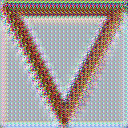
\includegraphics[height=\textwidth]{../images/snow generation/5.png}
  \end{subfigure}
 \caption{Generierte Bilder des \ac{CycleGAN} mit Schnee}
 \label{fig:snow-imgs-unet}
 \end{figure}

 Abbildung \ref{fig:snow-imgs-generated} im Anhang zeigt weitere verschneite Bilder, die durch das \ac{CycleGAN} generiert sind.